\documentclass[a4paper]{article}
\usepackage{geometry}
\usepackage{graphicx}
\usepackage{natbib}
\usepackage{amsmath}
\usepackage{amssymb}
\usepackage{amsthm}
\usepackage{paralist}
\usepackage{epstopdf}
\usepackage{tabularx}
\usepackage{longtable}
\usepackage{multirow}
\usepackage{multicol}
\usepackage[hidelinks]{hyperref}
\usepackage{fancyvrb}
\usepackage{algorithm}
\usepackage{algorithmic}
\usepackage{float}
\usepackage{paralist}
\usepackage[svgname]{xcolor}
\usepackage{enumerate}
\usepackage{array}
\usepackage{times}
\usepackage{url}
\usepackage{fancyhdr}
\usepackage{comment}
\usepackage{environ}
\usepackage{times}
\usepackage{textcomp}
\usepackage{caption}
\usepackage{multirow}
\usepackage{multicol}
\usepackage{floatrow}
\usepackage{amsmath}
\usepackage[makeroom]{cancel}


\urlstyle{rm}

\setlength\parindent{0pt} % Removes all indentation from paragraphs
\theoremstyle{definition}
\newtheorem{definition}{Definition}[]
\newtheorem{conjecture}{Conjecture}[]
\newtheorem{example}{Example}[]
\newtheorem{theorem}{Theorem}[]
\newtheorem{lemma}{Lemma}
\newtheorem{proposition}{Proposition}
\newtheorem{corollary}{Corollary}


\floatname{algorithm}{Procedure}
\renewcommand{\algorithmicrequire}{\textbf{Input:}}
\renewcommand{\algorithmicensure}{\textbf{Output:}}
\newcommand{\abs}[1]{\lvert#1\rvert}
\newcommand{\norm}[1]{\lVert#1\rVert}
\newcommand{\RR}{\mathbb{R}}
\newcommand{\CC}{\mathbb{C}}
\newcommand{\Nat}{\mathbb{N}}
\newcommand{\br}[1]{\{#1\}}
\DeclareMathOperator*{\argmin}{arg\,min}
\DeclareMathOperator*{\argmax}{arg\,max}
\renewcommand{\qedsymbol}{$\blacksquare$}

\definecolor{dkgreen}{rgb}{0,0.6,0}
\definecolor{gray}{rgb}{0.5,0.5,0.5}
\definecolor{mauve}{rgb}{0.58,0,0.82}

\newcommand{\Var}{\mathrm{Var}}
\newcommand{\Cov}{\mathrm{Cov}}

\newcommand{\vc}[1]{\boldsymbol{#1}}
\newcommand{\xv}{\vc{x}}
\newcommand{\Sigmav}{\vc{\Sigma}}
\newcommand{\alphav}{\vc{\alpha}}
\newcommand{\muv}{\vc{\mu}}

\newcommand{\red}[1]{\textcolor{red}{#1}}

\def\x{\mathbf x}
\def\y{\mathbf y}
\def\w{\mathbf w}
\def\v{\mathbf v}
\def\E{\mathbb E}
\def\V{\mathbb V}

% TO SHOW SOLUTIONS, include following (else comment out):
\newenvironment{soln}{
    \leavevmode\color{blue}\ignorespaces
}{}


\hypersetup{
%    colorlinks,
    linkcolor={red!50!black},
    citecolor={blue!50!black},
    urlcolor={blue!80!black}
}

\geometry{
  top=1in,            % <-- you want to adjust this
  inner=1in,
  outer=1in,
  bottom=1in,
  headheight=3em,       % <-- and this
  headsep=2em,          % <-- and this
  footskip=3em,
}


\pagestyle{fancyplain}
\lhead{\fancyplain{}{Homework 3}}
\rhead{\fancyplain{}{CS 760 Machine Learning}}
\cfoot{\thepage}

\title{\textsc{Homework 3}} % Title

%%% NOTE:  Replace 'NAME HERE' etc., and delete any "\red{}" wrappers (so it won't show up as red)

\author{
\red{Matt Myers} \\
\red{908-464-4252}\\
\red{\href{https://github.com/myersmt/Hw003-Comp760}{GitHub}}\\
} 

\date{}

\begin{document}

\maketitle 


\textbf{Instructions:} 
Use this latex file as a template to develop your homework. Submit your homework on time as a single pdf file to Canvas. Late submissions may not be accepted. Please wrap your code and upload to a public GitHub repo, then attach the link below the instructions so that we can access it. You can choose any programming language (i.e. python, R, or MATLAB). Please check Piazza for updates about the homework.

\section{Questions (50 pts)}
\begin{enumerate}
\item (9 pts) Explain whether each scenario is a classification or regression problem. And, provide the number of data points ($n$) and the number of features ($p$).

\begin{enumerate}
	\item (3 pts) We collect a set of data on the top 500 firms in the US. For each firm we record profit, number of employees, industry and the CEO salary. We are interested in predicting CEO salary with given factors.\\
	
	\begin{soln}
            This is a prime example of a regression problem. There is 500 data points ($n = 500$) with three features each ($p = 3$). These features are, profit, number of employees, and industry.
        \end{soln}\\
	
	\item (3 pts) We are considering launching a new product and wish to know whether it will be a success or a failure. We collect data on 20 similar products that were previously launched. For each product we have recorded the price charged for the product, marketing budget, competition price, and ten other variables. These add up to be 13 total features\\
	
	\begin{soln}
            This is a classification problem. The 20 similar products make up our 20 data points ($n = 20$). There are thirteen features as described there is success or failure, price change, marketing budget, competition price, and then ten other variables ($p = 13$).
        \end{soln}\\
	
	\item (3 pts) We are interesting in predicting the \% change in the US dollar in relation to the weekly changes in the world stock markets. Hence we collect weekly data for all of 2012. For each week we record the \% change in the dollar, the \% change in the US market, the \% change in the British market, and the \% change in the German market.\\
	
	\begin{soln}
            This is a regression problem. The number of data points is equal to the number of weeks in 2012 which was 52 ($n = 52$). There are three features that go with this, the \% change in the US market, the \% change in the British market, and the \% change in the German Market ($p = 3$).
        \end{soln}\\
	
\end{enumerate}

\item (6 pts) The table below provides a training data set containing six observations, three predictors, and one qualitative response variable.

\begin{center}
	\begin{tabular}{ c  c  c  c}
		\hline
		$X_{1}$ & $X_{2}$ & $X_{3}$ & $Y$ \\ \hline
		0 & 3 & 0 & Red \\
		2 & 0 & 0 & Red \\
		0 & 1 & 3 & Red \\
		0 & 1 & 2 & Green \\
		-1 & 0 & 1 & Green \\
		1 & 1 & 1 & Red  \\
		\hline
	\end{tabular}
\end{center}

Suppose we wish to use this data set to make a prediction for $Y$ when $X_{1} = X_{2} = X_{3} = 0$ using K-nearest neighbors.

\begin{enumerate}
	\item (2 pts) Compute the Euclidean distance between each observation and the test point, $X_{1} = X_{2} = X_{3}=0$.\\
 
	\begin{soln}
            Note that Euclidean distance is calculated with the formula $d = \sqrt{X^2_1 + X^2_2 + X^2_3}$. Because $X_1 = X_2 = X_3 = 0$, the starting Euclidean distance $d = (0,0,0)$.\\\\
            $d_1 = \sqrt{0^2 + 3^2 + 0^2} = \sqrt{9} = 3$\qquad \qquad \quad
            $d_2 = \sqrt{2^2 + 0^2 + 0^2} = \sqrt{4} = 2$\\
            $d_3 = \sqrt{0^2 + 1^2 + 3^2} = \sqrt{10} \approx 3.162$\qquad \quad
            $d_4 = \sqrt{0^2 + 1^2 + 2^2} = \sqrt{5} \approx  2.236$\\
            $d_5 = \sqrt{-1^2 + 0^2 + 1^2} = \sqrt{2} \approx 1.414$\qquad \quad
            $d_6 = \sqrt{1^2 + 1^2 + 1^2} = \sqrt{3} \approx 1.732$\\\\
            \begin{center}
	\begin{tabular}{ c  c  c  c  c}
		\hline
		$X_{1}$ & $X_{2}$ & $X_{3}$ & $Y$ & $d$\\ \hline
		0 & 3 & 0 & Red & 3\\
		2 & 0 & 0 & Red & 2\\
		0 & 1 & 3 & Red & $\sqrt{10}$\\
		0 & 1 & 2 & Green & $\sqrt{5}$\\
		-1 & 0 & 1 & Green & $\sqrt{2}$\\
		1 & 1 & 1 & Red & $\sqrt{3}$\\
		\hline
	\end{tabular}
        \end{center}
        \end{soln}\\\\
 \\
	\item (2 pts) What is our prediction with $K=1$? Why?\\
	
	\begin{soln}
            For $K = 1$ the best prediction is $Y =$ Green. This is because the smallest distance is in observation 5, where $d = \sqrt{2} \approx 1.414$. This means that the nearest neighbor is the fifth observation which has label $Y =$ Green. 
        \end{soln}\\
	
	\item (2 pts) What is our prediction with $K=3$? Why?\\
	
	\begin{soln}
            For $K = 3$ we take the three nearest neighbors which leads us to the prediction $Y =$ Red. The three nearest neighbors are observations 5, 6, and 2 in that order. The most common label amongst those three results is $Y =$ Red. That is how the prediction is found.
        \end{soln}\\

\end{enumerate}

\item (12 pts) When the number of features $p$ is large, there tends to be a deterioration in the performance of KNN and other local approaches that perform prediction using only observations that are near the test ob- servation for which a prediction must be made. This phenomenon is known as the curse of dimensionality, and it ties into the fact that non-parametric approaches often perform poorly when $p$ is large.

\begin{enumerate}
	\item (2pts) Suppose that we have a set of observations, each with measurements on $p=1$ feature, $X$. We assume that $X$ is uniformly (evenly) distributed on [0, 1]. Associated with each observation is a response value. Suppose that we wish to predict a test observation’s response using only observations that are within 10\% of the range of $X$ closest to that test observation. For instance, in order to predict the response for a test observation with $X=0.6$, we will use observations in the range [0.55, 0.65]. On average, what fraction of the available observations will we use to make the prediction?
	\\\\
	\begin{soln}
            For a given test observation with value X, the range within 10\% would have to [X - 0.05, X + 0.05]. Since X is uniformly distributed on [0, 1] all intervals are equally likely meaning on average 10\% of the observations will be used to make predictions.
        \end{soln}\\
	
	
	\item (2pts) Now suppose that we have a set of observations, each with measurements on $p =2$ features, $X1$ and $X2$. We assume that predict a test observation’s response using only observations that $(X1,X2)$ are uniformly distributed on [0, 1] × [0, 1]. We wish to are within 10\% of the range of $X1$ and within 10\% of the range of $X2$ closest to that test observation. For instance, in order to predict the response for a test observation with $X1 =0.6$ and $X2 =0.35$, we will use observations in the range [0.55, 0.65] for $X1$ and in the range [0.3, 0.4] for $X2$. On average, what fraction of the available observations will we use to make the prediction?
	\\\\
	\begin{soln}
            For the range of $X_1$ that is within 10\% of 0.6 is [0.55, 0.65], and the range of $X_2$ that is within 10\% of 0.35 is [0.3, 0.4]. Since $X_1$ and $X_2$ are independent and uniformly distributed on [0, 1], the fraction of observations that fall within both ranges is equal to $\frac{0.1\cdot0.1}{1} = 0.01$. This means that on average we use 1\% of the available observations to make a prediction.
        \end{soln}\\
	
	\item (2pts) Now suppose that we have a set of observations on $p = 100$ features. Again the observations are uniformly distributed on each feature, and again each feature ranges in value from 0 to 1. We wish to predict a test observation’s response using observations within the 10\% of each feature’s range that is closest to that test observation. What fraction of the available observations will we use to make the prediction?
	\\\\
	\begin{soln}
            Using similar logic as the previous question, The range of each feature that is within 10\% of the test observation is [0.45, 0.55]. Since each feature is independent and uniformly distributed on [0, 1], the fraction of observations that fall within this range for each feature is equal to the product of all their ranges. This means that on average we will use $0.1^p = 0.1^{100} = 1 \cdot 10^{-100}$ of the available observation to make the prediction.
        \end{soln}\\
	
	\item (3pts) Using your answers to parts (a)–(c), argue that a drawback of KNN when p is large is that there are very few training observations “near” any given test observation.
	\\\\
	\begin{soln}
            In parts (a)-(c) we demonstrate that as $p$ increases, the fraction of observations that are "near" the test observation decreases. This means that there are very few training observations that are helpful for creating predictions for any test observation. This causes KNN to not work very well as $p$ becomes very large.
        \end{soln}\\
	
	\item (3pts) Now suppose that we wish to make a prediction for a test observation by creating a $p$-dimensional hypercube centered around the test observation that contains, on average, 10\% of the training observations. For $p =$1, 2, and 100, what is the length of each side of the hypercube? Comment on your answer.
	\\\\
	\begin{soln}
            For a hypercube with p-dimensions centered around the test observation we can create a fairly simple equation for calculating the length of each side of the hypercube. This equation would be $l = 0.1^{\frac{1}{p}}$. This could be seen with part (c), therefore for the calculations for each p, we have the following:\\\\
            $l_{p=1} = 0.1^{1} = 0.1$ \\ 
            $l_{p=2} = 0.1^{\frac{1}{2}} = \sqrt{0.1} = 0.316$ \\
            $l_{p=100} = 0.1^{\frac{1}{100}} = 0.9772$ \\\\
            These results show that to stay within a 10\% threshold of the observations used in the prediction, we have to keep incorporating points further and further away.
        \end{soln}\\
	
\end{enumerate}

\item (6 pts) Supoose you trained a classifier for a spam detection system. The prediction result on the test set is summarized in the following table.
\begin{center}
	\begin{tabular}{l l | l l}
		&          & \multicolumn{2}{l}{Predicted class} \\
		&          & Spam           & not Spam           \\
		\hline
		\multirow{2}{*}{Actual class} & Spam     & 8              & 2                  \\
		& not Spam & 16             & 974               
	\end{tabular}
\end{center}

Calculate
\begin{enumerate}
	\item (2 pts) Accuracy\\
    	\begin{soln}
                The accuracy has to do with how many were predicted that were correct this can be found by the total correct divided by the total. In this case that would be $\frac{8+974}{1000} = \frac{982}{1000} = 0.982 = 98.2\%$.
            \end{soln}
	\item (2 pts) Precision\\
            \begin{soln}
                The precision is based on how precisely it predicted the spam out of the emails. In this example it found 8 spam that were actually spam but improperly flagged 16 emails as spam that weren't. This leads to the precision being $\frac{8}{8+16} = \frac{8}{24} = \frac{1}{3} = 0.3\bar{3} = 33.3\bar{3}\%$.
            \end{soln}
	\item (2 pts) Recall\\
		\begin{soln}
                Recall has to do with the actual spam that was predicted to be spam versus the spam that was not found to be spam. For this example there was ten total spam emails. Eight were correctly identified and two snuck through. This leads are recall to be $\frac{8}{8+2} = \frac{8}{10} = \frac{4}{5} = 0.8 = 80\%$.
            \end{soln}
\end{enumerate}


\item (9pts) Again, suppose you trained a classifier for a spam filter. The prediction result on the test set is summarized in the following table. Here, "+" represents spam, and "-" means not spam.

\begin{center}
\begin{tabular}{ c  c }
\hline
Confidence positive & Correct class \\ \hline
0.95 & + \\
0.85 & + \\
0.8 & - \\
0.7 & + \\
0.55 & + \\
0.45 & - \\
0.4 & + \\
0.3 & + \\
0.2 & - \\
0.1 & - \\
\hline
\end{tabular}
\end{center}

\begin{enumerate}
	\item (6pts) Draw a ROC curve based on the above table.
	\begin{soln}
            \begin{figure}[H]
                \centering
                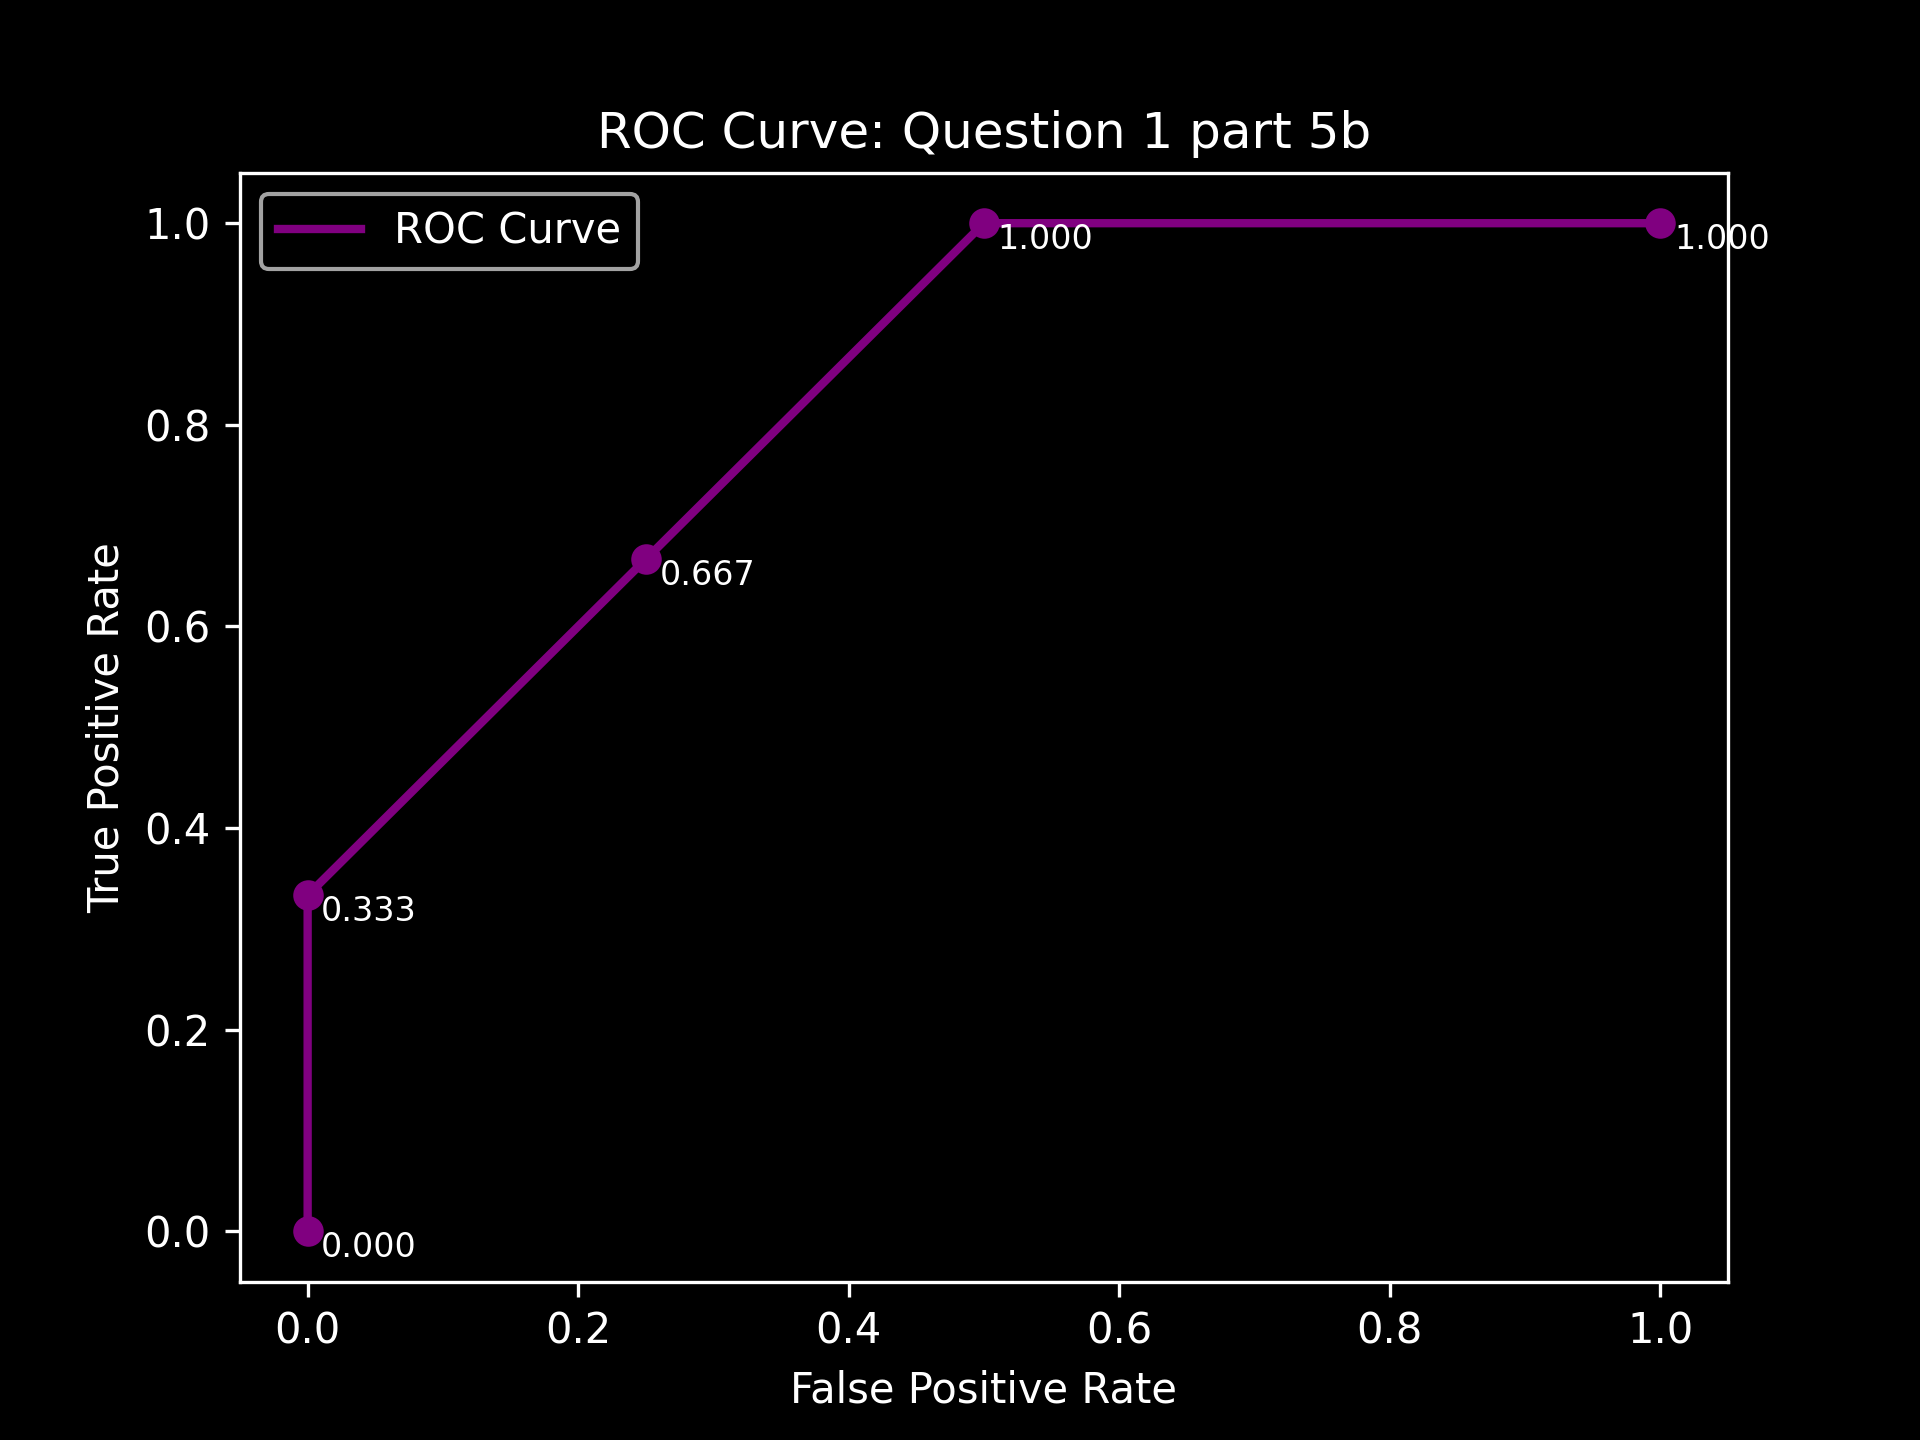
\includegraphics[width=0.75\textwidth]{figs/q1/p5/q1-p5roc_curve_q1-p5b.png} 
                \captionsetup{labelformat=empty}
                \caption{}
                \label{fig:my_label}
             \end{figure}
        \end{soln}
	
	\item (3pts) (Real-world open question) Suppose you want to choose a threshold parameter so that mails with confidence positives above the threshold can be classified as spam. Which value will you choose? Justify your answer based on the ROC curve.\\
	
	\begin{soln}
            Looking at the chart  I believe that it would depend on what the user values more. The only way to get zero false positives would be to also get zero true positives at which point the spam is not even being filtered. I believe a good sweet spot would either be 0.45 or 0.2 depending on how aggressive you would want. If you value having no spam then at 0.45 false positive rate 100\% accurate filtering is achieved. However for the sake of not missing possible important emails I feel that I would go with the 0.2 false positive rate. Only getting 1 out of every 5 false positives while getting nearly 50\% of all the spam emails. I think this question does boil down to preference however.
        \end{soln}\\
\end{enumerate}

\item (8 pts) In this problem, we will walk through a single step of the gradient descent algorithm for logistic regression. As a reminder,
$$f(x;\theta) = \sigma(\theta^\top x)$$
$$\text{Cross entropy loss } L(\hat{y}, y) = -[y \log  \hat{y} + (1-y)\log(1-\hat{y})]$$
$$\text{The single update step } \theta^{t+1} = \theta^{t} - \eta \nabla_{\theta} L(f(x;\theta), y) $$



\begin{enumerate}
	\item (4 pts) Compute the first gradient $\nabla_{\theta} L(f(x;\theta), y)$.
	
	\begin{soln}
            \begin{align*}
                \triangledown_\theta L(f(x;\theta),y) &= \triangledown_\theta[-y\log(\sigma(\theta^Tx))-(1-y)\log(1-\sigma(\theta^Tx))]\\
                &= \frac{-y}{\sigma(\theta^Tx)}\cdot\sigma'(\theta^Tx)\cdot x-\frac{1-y}{1-\sigma(\theta^Tx)}\cdot\sigma'(\theta^Tx)\cdot x\\
                &= -y\cdot(1-\sigma(\theta^Tx))\cdot x-1+y\cdot\sigma(\theta^Tx)\cdot x\\
                & = x(\sigma(\theta^Tx)-y)
                \end{align*}
        \end{soln}
	
	\item (4 pts)
 Now assume a two dimensional input. After including a bias parameter for the first dimension, we will have $\theta\in\mathbb{R}^3$.
$$ \text{Initial parameters : }  \theta^{0}=[0, 0, 0]$$
$$ \text{Learning rate }\eta=0.1$$
$$ \text{data example : } x=[1, 3, 2], y=1$$
Compute the updated parameter vector $\theta^{1}$ from the single update step.
	
	\begin{soln}
            \begin{align*}
                \theta^1 &= \theta^0 - \eta\cdot x(\sigma((\theta^0)^T\cdot x)-y)\\
                &= \theta^0 - 0.1\cdot[1,3,2](\sigma([0,0,0]^T[1,3,2])-1)\\
                &= \theta^0 - 0.1\cdot[1,3,2](\sigma(0)-1)\\
                &= \theta^0 - 0.1\cdot[1,3,2](\frac{1}{2})-1)\\
                &= \theta^0 - 0.1\cdot[1,3,2](-\frac{1}{2})\\
                &= [0,0,0] + \frac{1}{20}\cdot[1,3,2]\\
                &= [\frac{1}{20}, \frac{3}{20}, \frac{1}{10}]\\\\
                &= [0.05, 0.15, 0.10]
            \end{align*}
        \end{soln}
\end{enumerate}
\end{enumerate}

\section{Programming (50 pts)}
\begin{enumerate}
	\item (10 pts) Use the whole D2z.txt as training set.  Use Euclidean distance (i.e. $A=I$).
	Visualize the predictions of 1NN on a 2D grid $[-2:0.1:2]^2$.
	That is, you should produce test points whose first feature goes over $-2, -1.9, -1.8, \ldots, 1.9, 2$, so does the second feature independent of the first feature.
	You should overlay the training set in the plot, just make sure we can tell which points are training, which are grid.
	
	The expected figure looks like this.
	\begin{figure}[h]
		\centering
		\includegraphics[width=5cm]{needed/implementation1_expected_result.png}
	\end{figure}
 	\begin{soln}
            \begin{figure}[H]
                \centering
                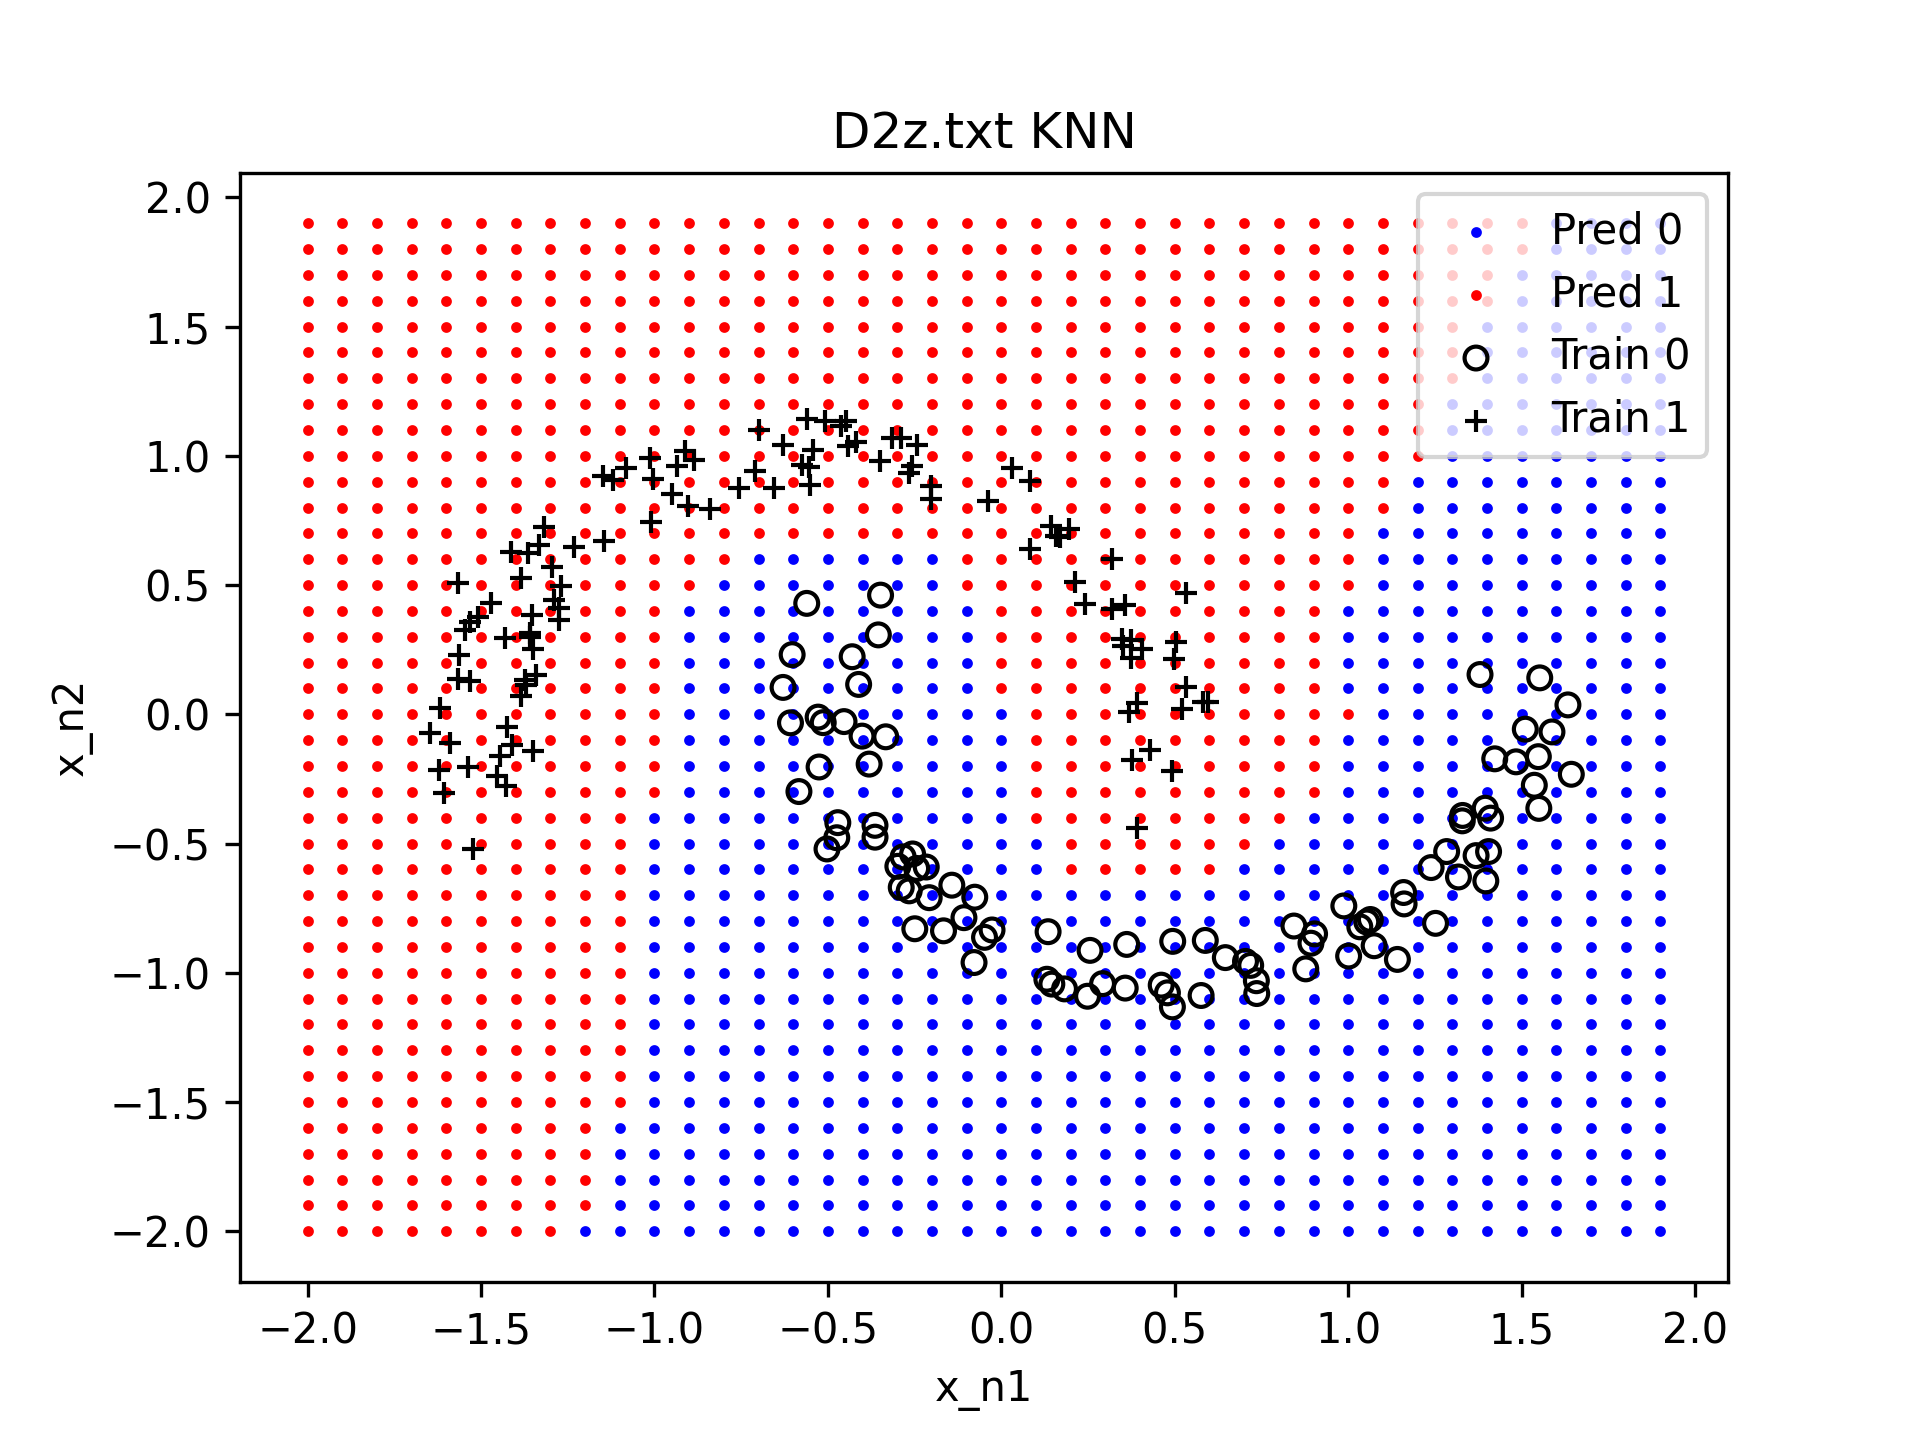
\includegraphics[width=0.75\textwidth]{figs/q2/p1/D2z.txt_KNN.png} 
                \captionsetup{labelformat=empty}
                \caption{}
                \label{fig:my_label}
             \end{figure}
        \end{soln}
	
	\paragraph{Spam filter} Now, we will use 'emails.csv' as our dataset. The description is as follows.
	\begin{figure}[h]
		\centering
		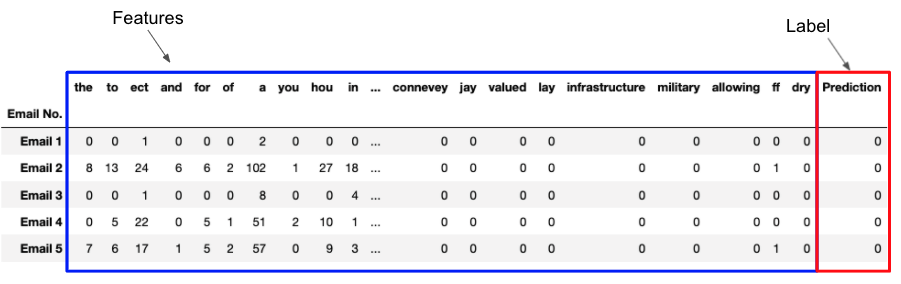
\includegraphics[width=\linewidth]{needed/email_head.png}
	\end{figure}
	
	\begin{itemize}
		\item Task: spam detection
		\item The number of rows: 5000
		\item The number of features: 3000 (Word frequency in each email)
		\item The label (y) column name: `Predictor'
		\item For a single training/test set split, use Email 1-4000 as the training set, Email 4001-5000 as the test set.
		\item For 5-fold cross validation, split dataset in the following way.
		\begin{itemize}
			\item Fold 1, test set: Email 1-1000, training set: the rest (Email 1001-5000)
			\item Fold 2, test set: Email 1000-2000, training set: the rest
			\item Fold 3, test set: Email 2000-3000, training set: the rest
			\item Fold 4, test set: Email 3000-4000, training set: the rest
			\item Fold 5, test set: Email 4000-5000, training set: the rest			
		\end{itemize}
	\end{itemize}
	
	\item (8 pts) Implement 1NN, Run 5-fold cross validation. Report accuracy, precision, and recall in each fold.
	
	\begin{soln}
             \begin{table}[H]
             \begin{soln}
                \begin{center}
                \begin{tabular}{c|c|c|c}
                \hline
                \textbf{Fold} & \textbf{Accuracy} & \textbf{Precision} & \textbf{Recall}\\ \hline
                1 & 0.825 & 0.65449 & 0.81754 \\ 
                2 & 0.853 & 0.68571 & 0.86643 \\ 
                3 & 0.862 & 0.72121 & 0.83803 \\ 
                4 & 0.851 & 0.71642 & 0.81633 \\ 
                5 & 0.775 & 0.60574 & 0.75817 \\ \hline
                \end{tabular}
                \end{center}
            \end{soln}
             \end{table}
        \end{soln}
	
	\item (12 pts) Implement logistic regression (from scratch). Use gradient descent (refer to question 6 from part 1) to find the optimal parameters. You may need to tune your learning rate to find a good optimum. Run 5-fold cross validation. Report accuracy, precision, and recall in each fold.
	
	\begin{soln}
            The Learning rate = 0.1, and the number of iterations = 1000.
             \begin{table}[H]
             \begin{soln}
                \begin{center}
                \begin{tabular}{c|c|c|c}
                \hline
                \textbf{Fold} & \textbf{Accuracy} & \textbf{Precision} & \textbf{Recall}\\ \hline
                1 & 0.909 & 0.89113 & 0.77544 \\ 
                2 & 0.854 & 0.90184 & 0.53069 \\ 
                3 & 0.889 & 0.82156 & 0.77817 \\ 
                4 & 0.843 & 0.66348 & 0.94558 \\ 
                5 & 0.849 & 0.78598 & 0.69608 \\ \hline
                \end{tabular}
                \end{center}
            \end{soln}
             \end{table}
        \end{soln}
	
	\item (10 pts) Run 5-fold cross validation with kNN varying k (k=1, 3, 5, 7, 10). Plot the average accuracy versus k, and list the average accuracy of each case. \\
	Expected figure looks like this.
	\begin{figure}[h]
		\centering
		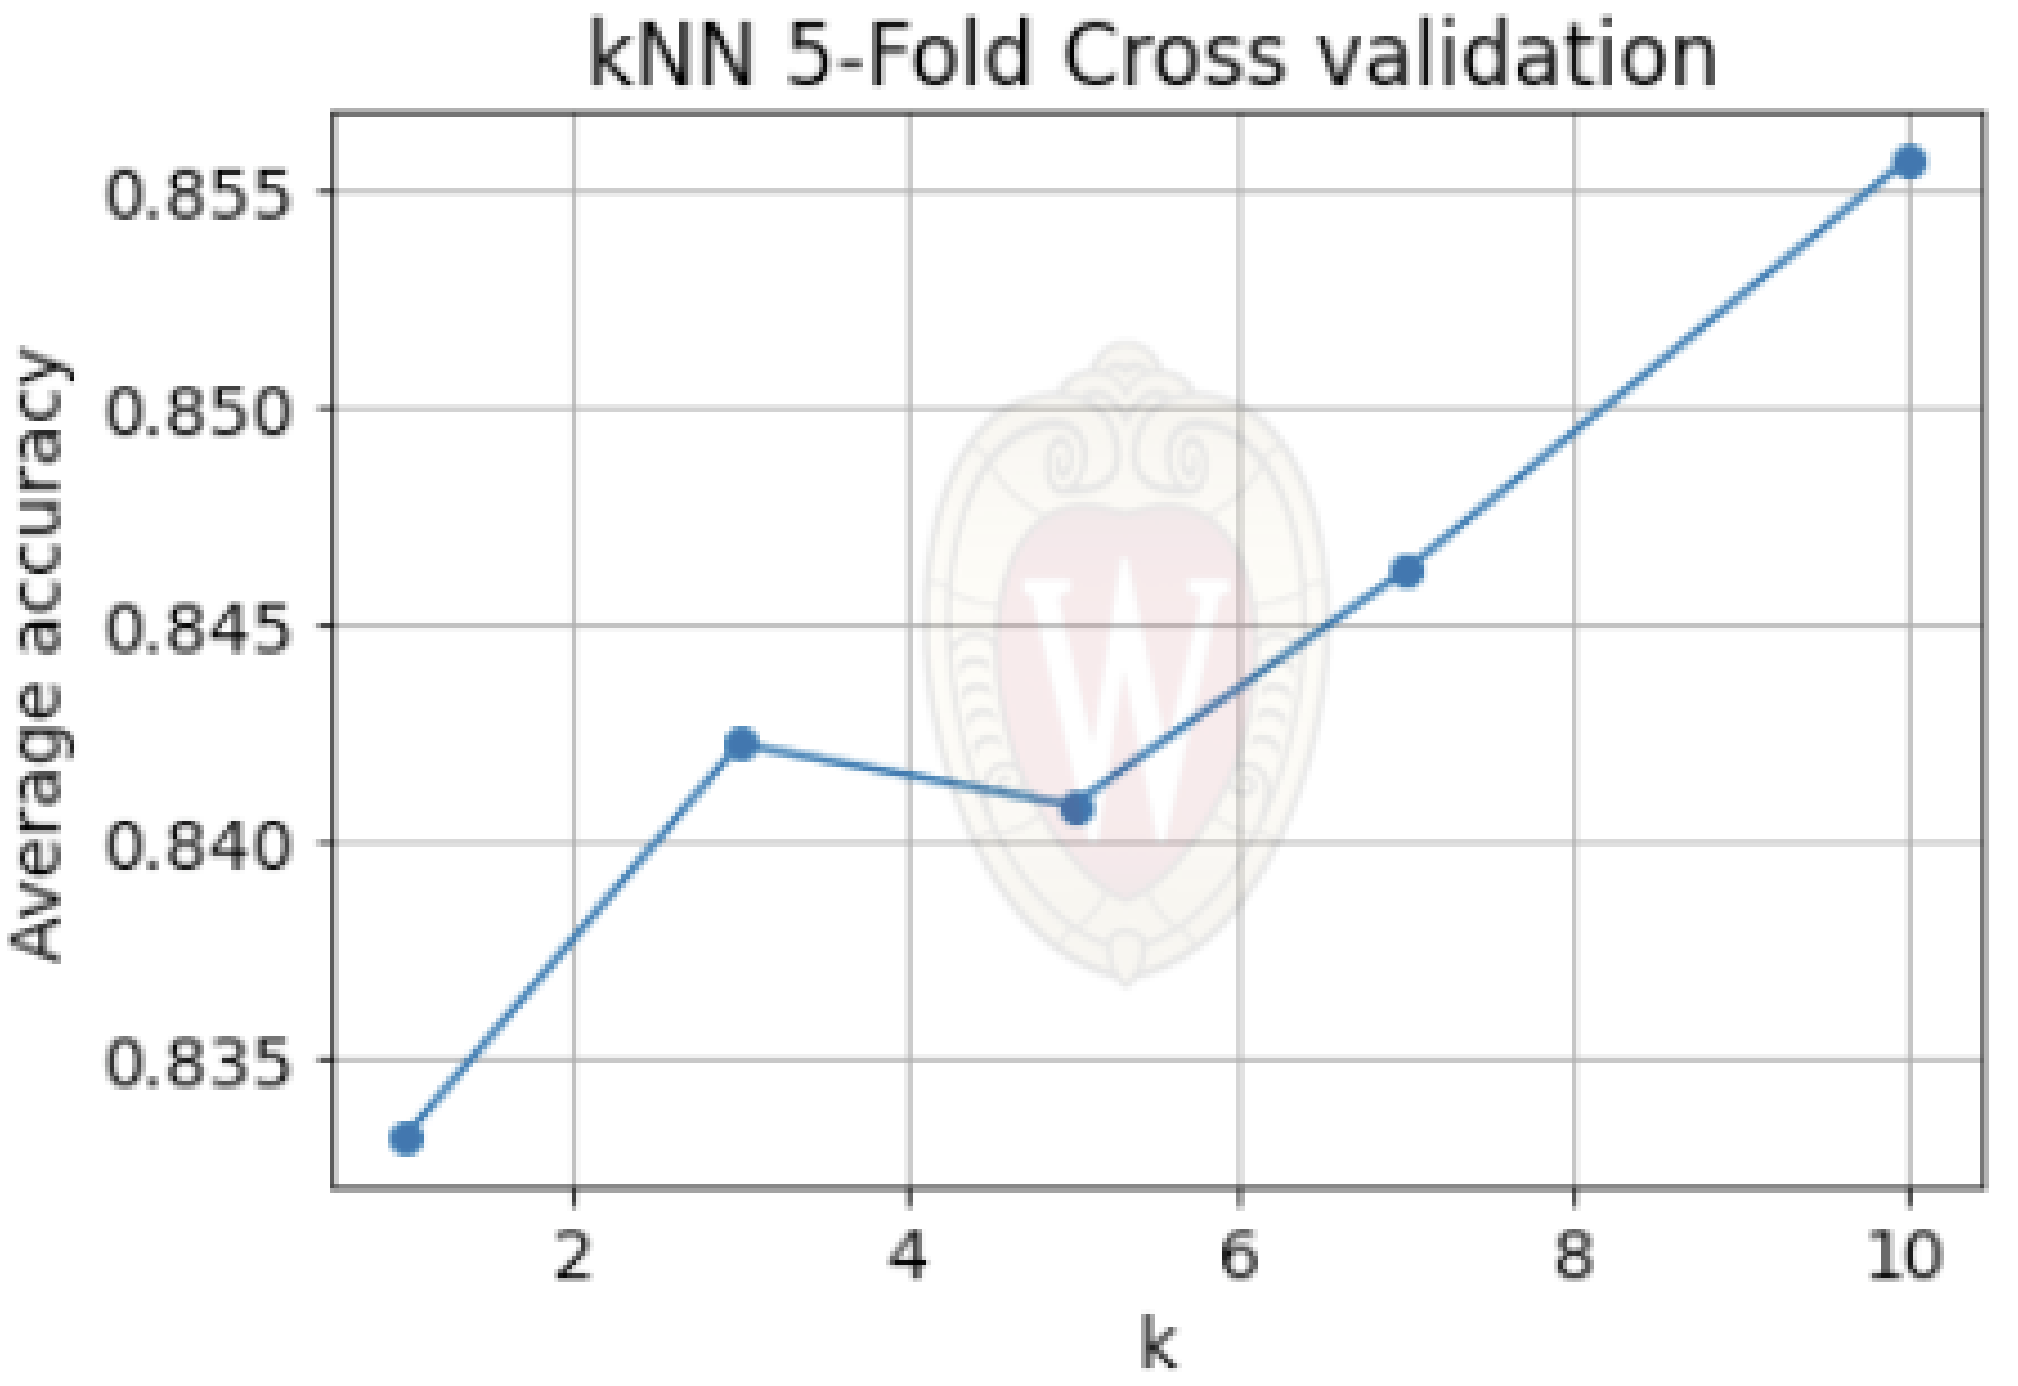
\includegraphics[width=8cm]{needed/knn.png}
	\end{figure}
	
	\begin{soln}
             \begin{table}[H]
                \begin{soln}
                \begin{center}
                \begin{tabular}{c|c}
                \hline
                \textbf{k} & \textbf{Average Accuracy} \\ \hline
                1          & 0.8332                    \\ 
                3          & 0.8422                    \\ 
                5          & 0.8408                    \\ 
                7          & 0.8462                    \\ 
                10         & 0.8556                    \\ \hline
                \end{tabular}
             \end{center}
            \end{soln}
             \end{table}
             \centering The above chart houses the values for the figure below.
             \begin{figure}[H]
                \centering
                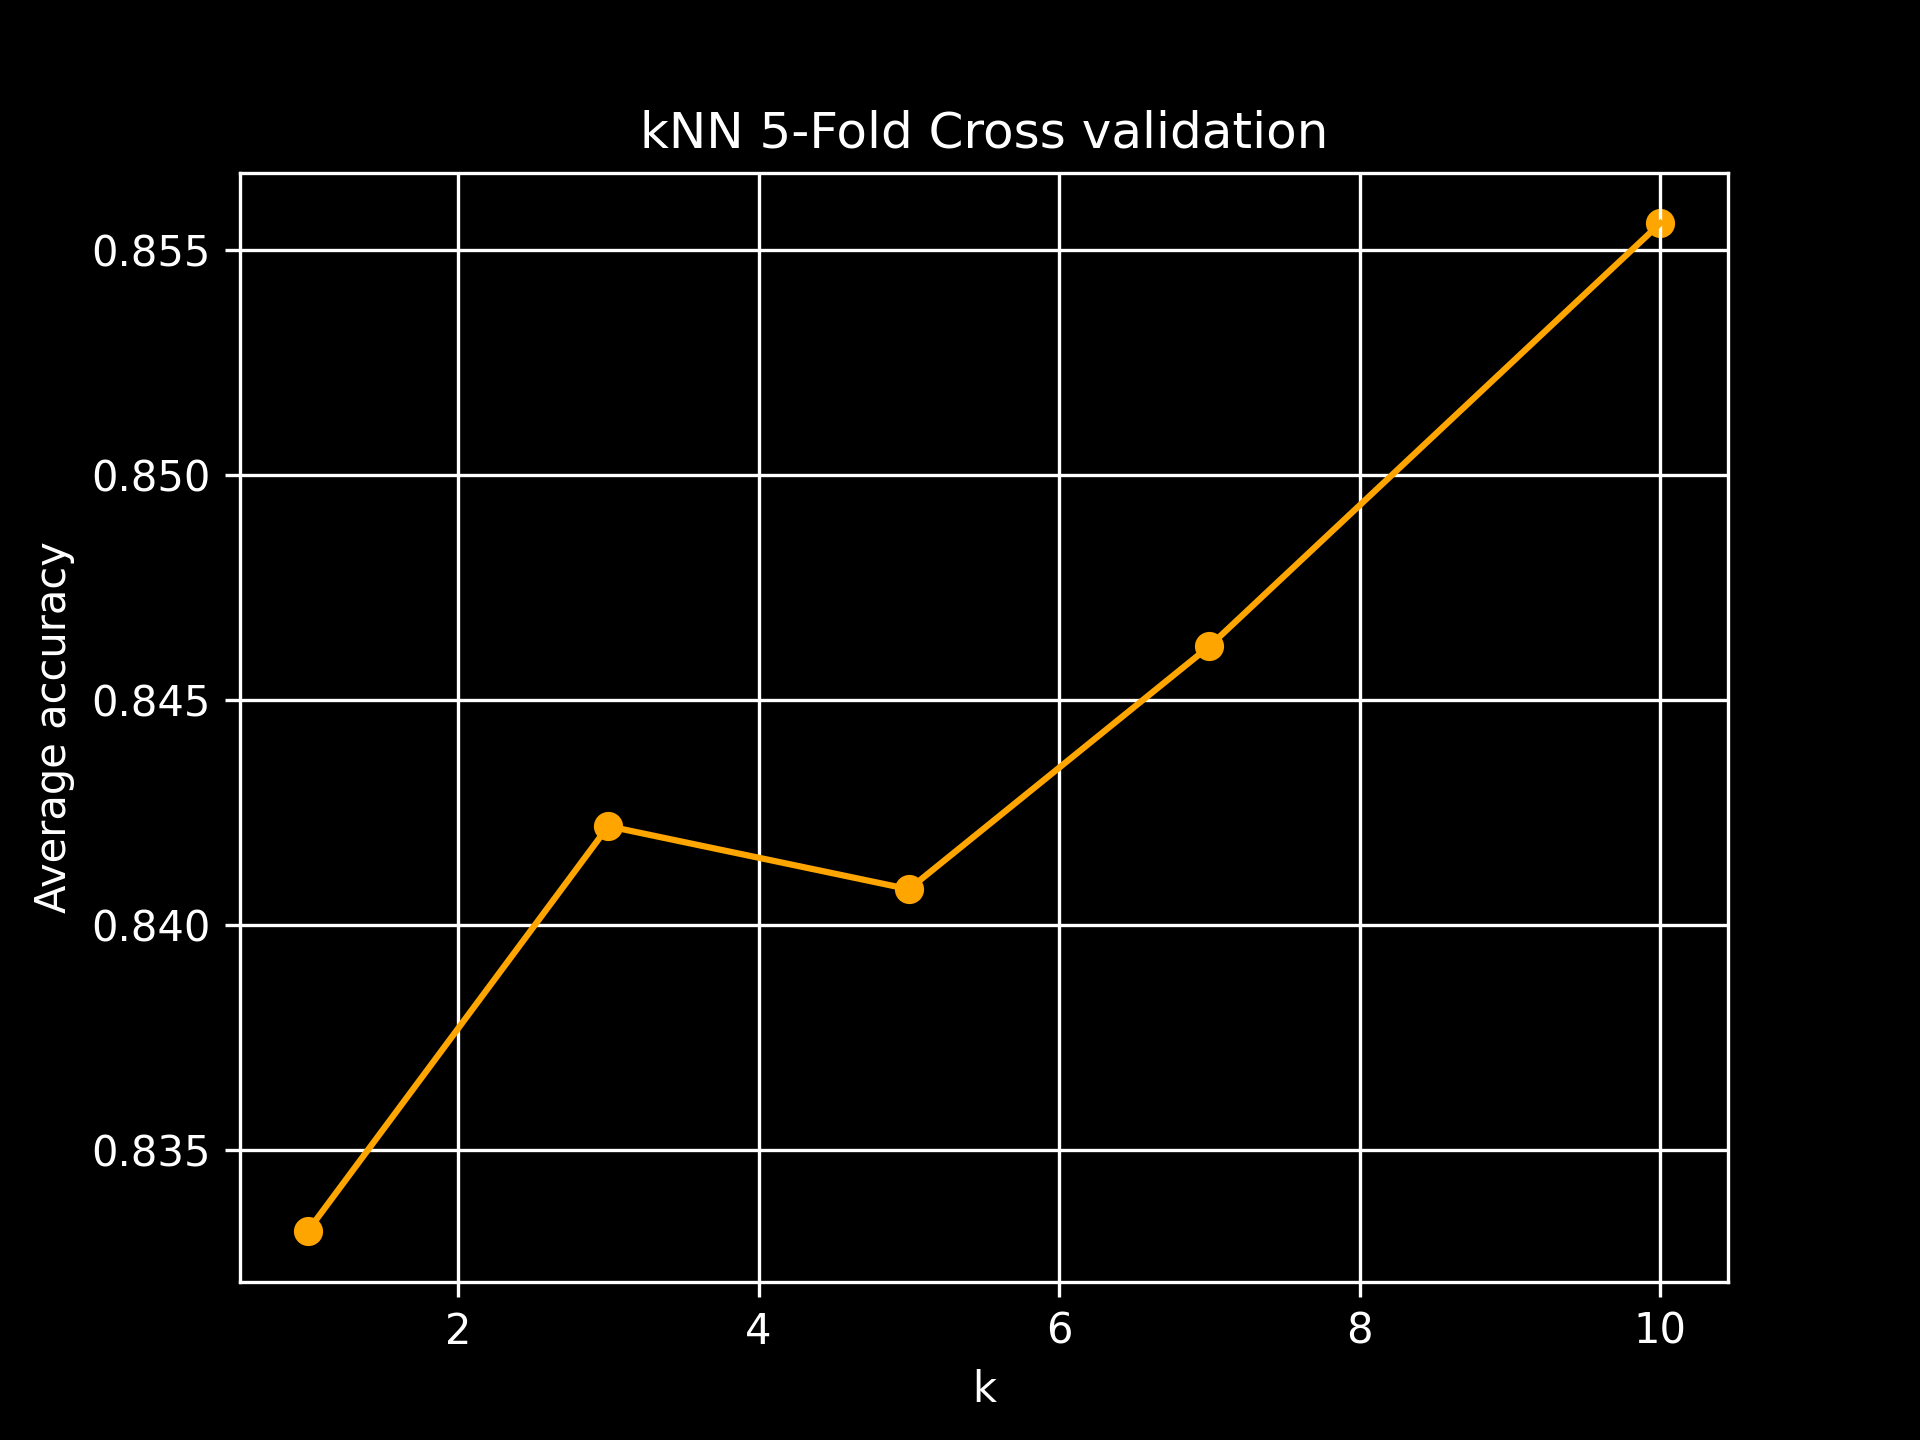
\includegraphics[width=0.5\textwidth]{figs/q2/p4/kNN_5-Fold_Cross_validation.png} 
                \captionsetup{labelformat=empty}
                \caption{}
                \label{fig:my_label}
             \end{figure}
        \end{soln}
	
	\item (10 pts) Use a single training/test setting. Train kNN (k=5) and logistic regression on the training set, and draw ROC curves based on the test set. \\
	Expected figure looks like this.
	\begin{figure}[h]
		\centering
		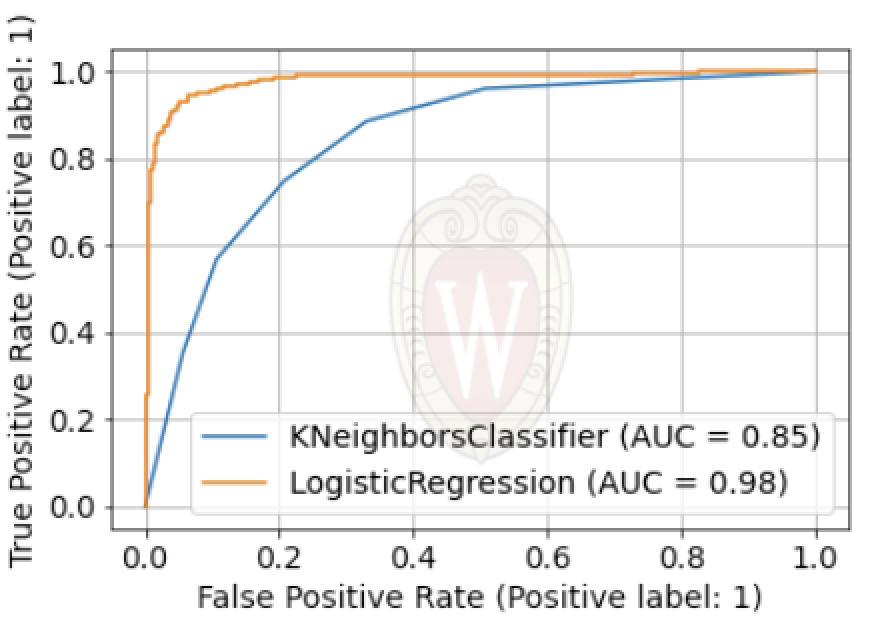
\includegraphics[width=8cm]{needed/roc.png}
	\end{figure}
	Note that the logistic regression results may differ.
	
	\begin{soln}
            \begin{figure}[H]
                \centering
                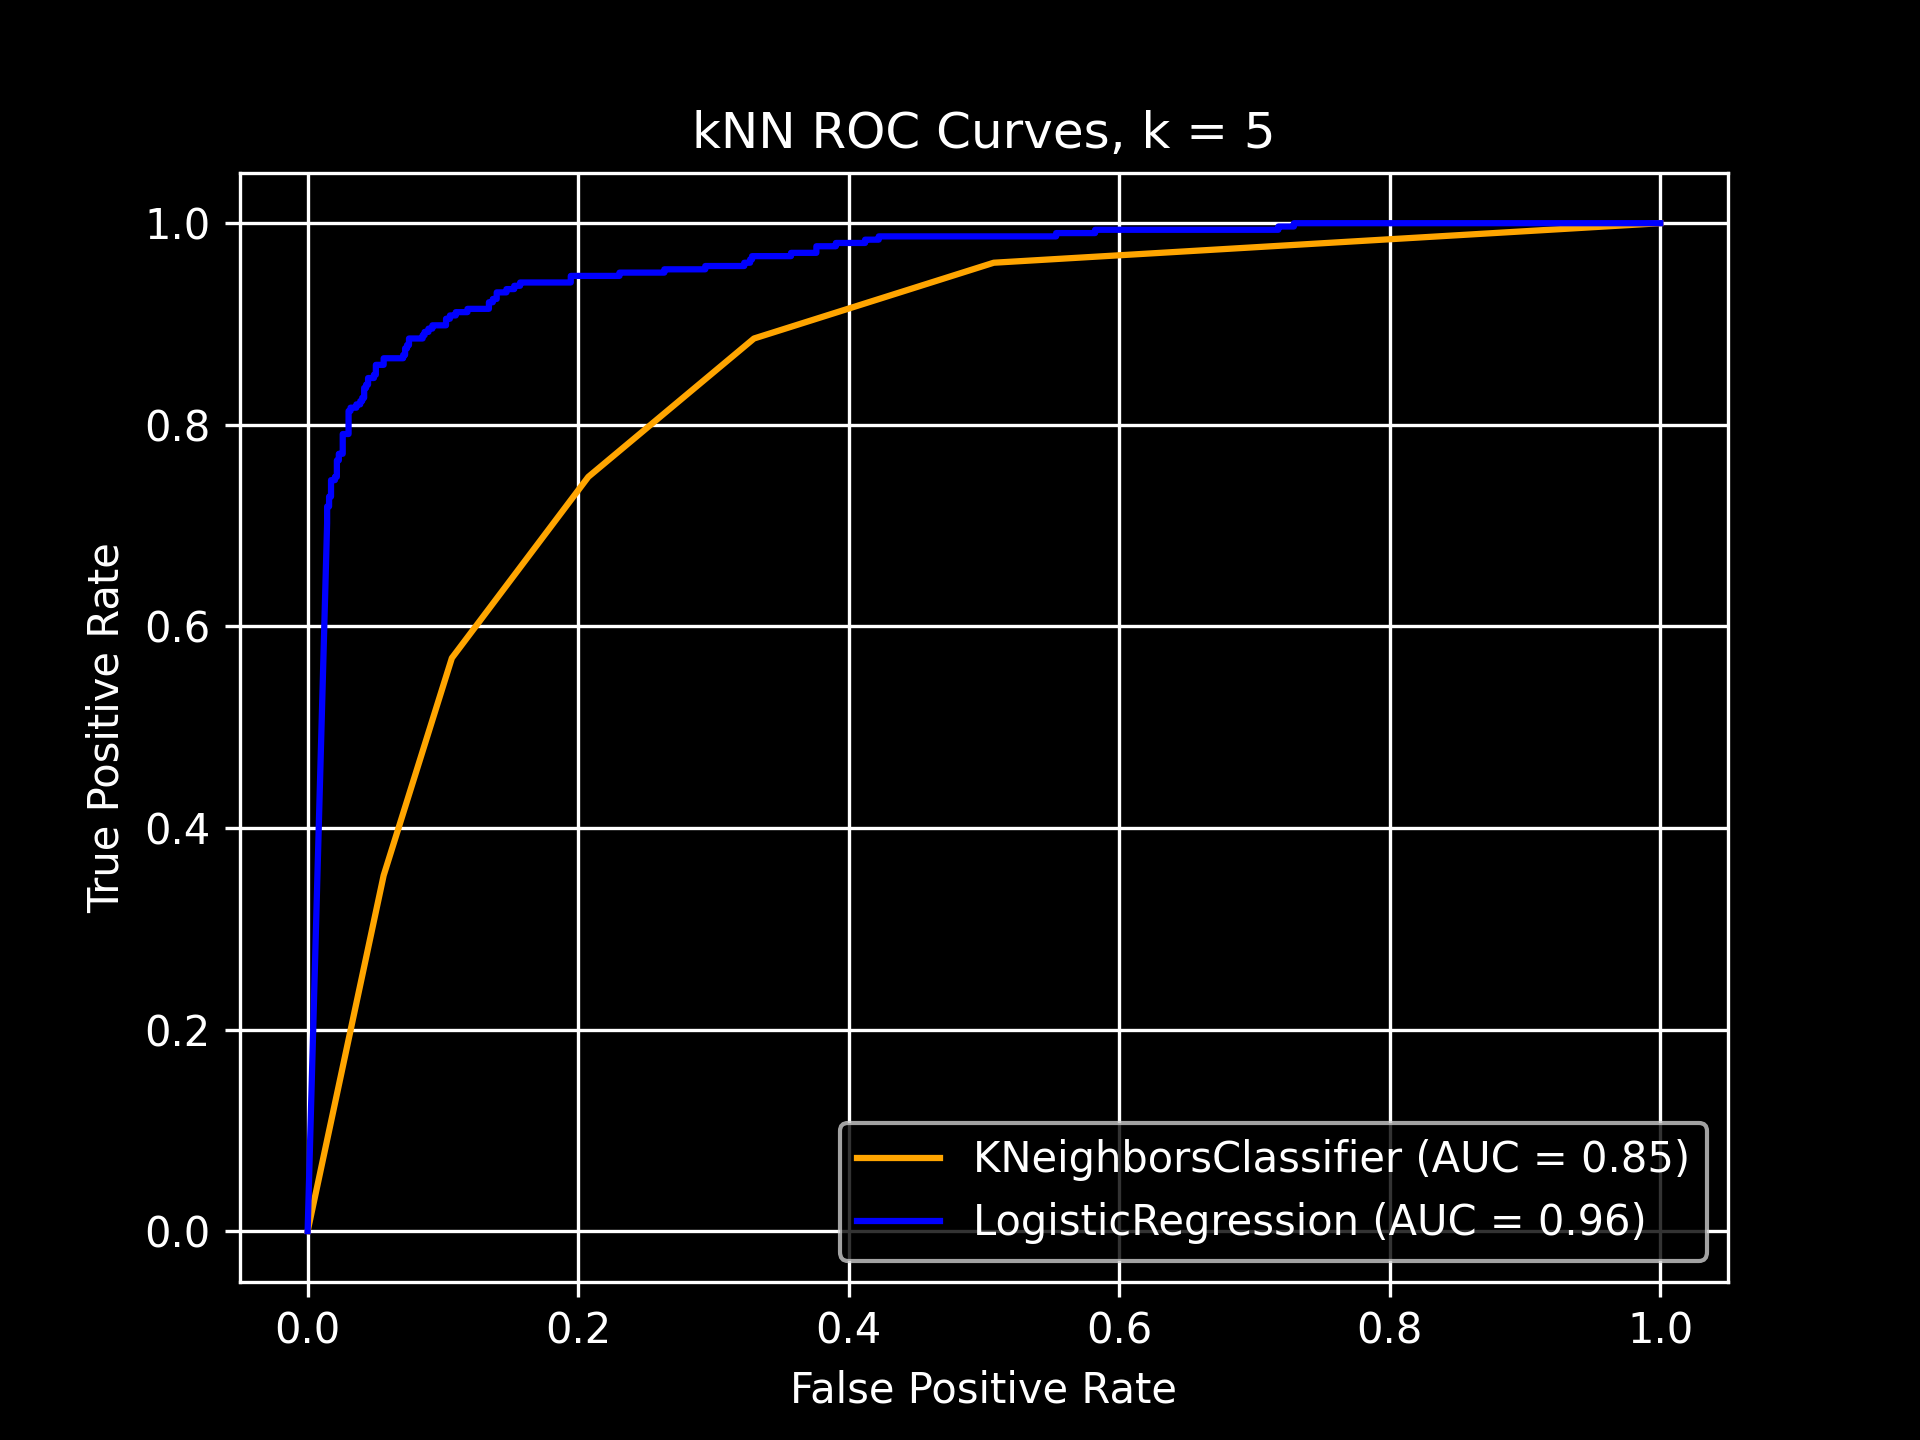
\includegraphics[width=0.6\textwidth]{figs/q2/p5/kNN_ROC_Curves.png} 
                \captionsetup{labelformat=empty}
                \caption{Learning rate = 0.1, Number of iterations = 10,000}
                \label{fig:my_label}
             \end{figure}
        \end{soln}
	
\end{enumerate}
\bibliographystyle{apalike}
\newpage
\red{\url{https://github.com/myersmt/Hw002-Comp760}}
\end{document}